%!TEX root = ../main.tex

\subsection{Geometric component}
\label{ss:geometric_component}

As may have become clear from the previous section, the only available information for the construction of the geometric component (and normal component) are the three vertices that define a single primitive. The vertices contain the vertex \textit{xyz} coordinates together with a unique normal per vertex i.e. the normals of each vertex is the same for every primitive using that vertex. Figure \ref{fig:method:input_primitive} contains an illustration of ``the input primitive'', which is the start point of the construction of every PN triangle.

\begin{figure}
	\centering
	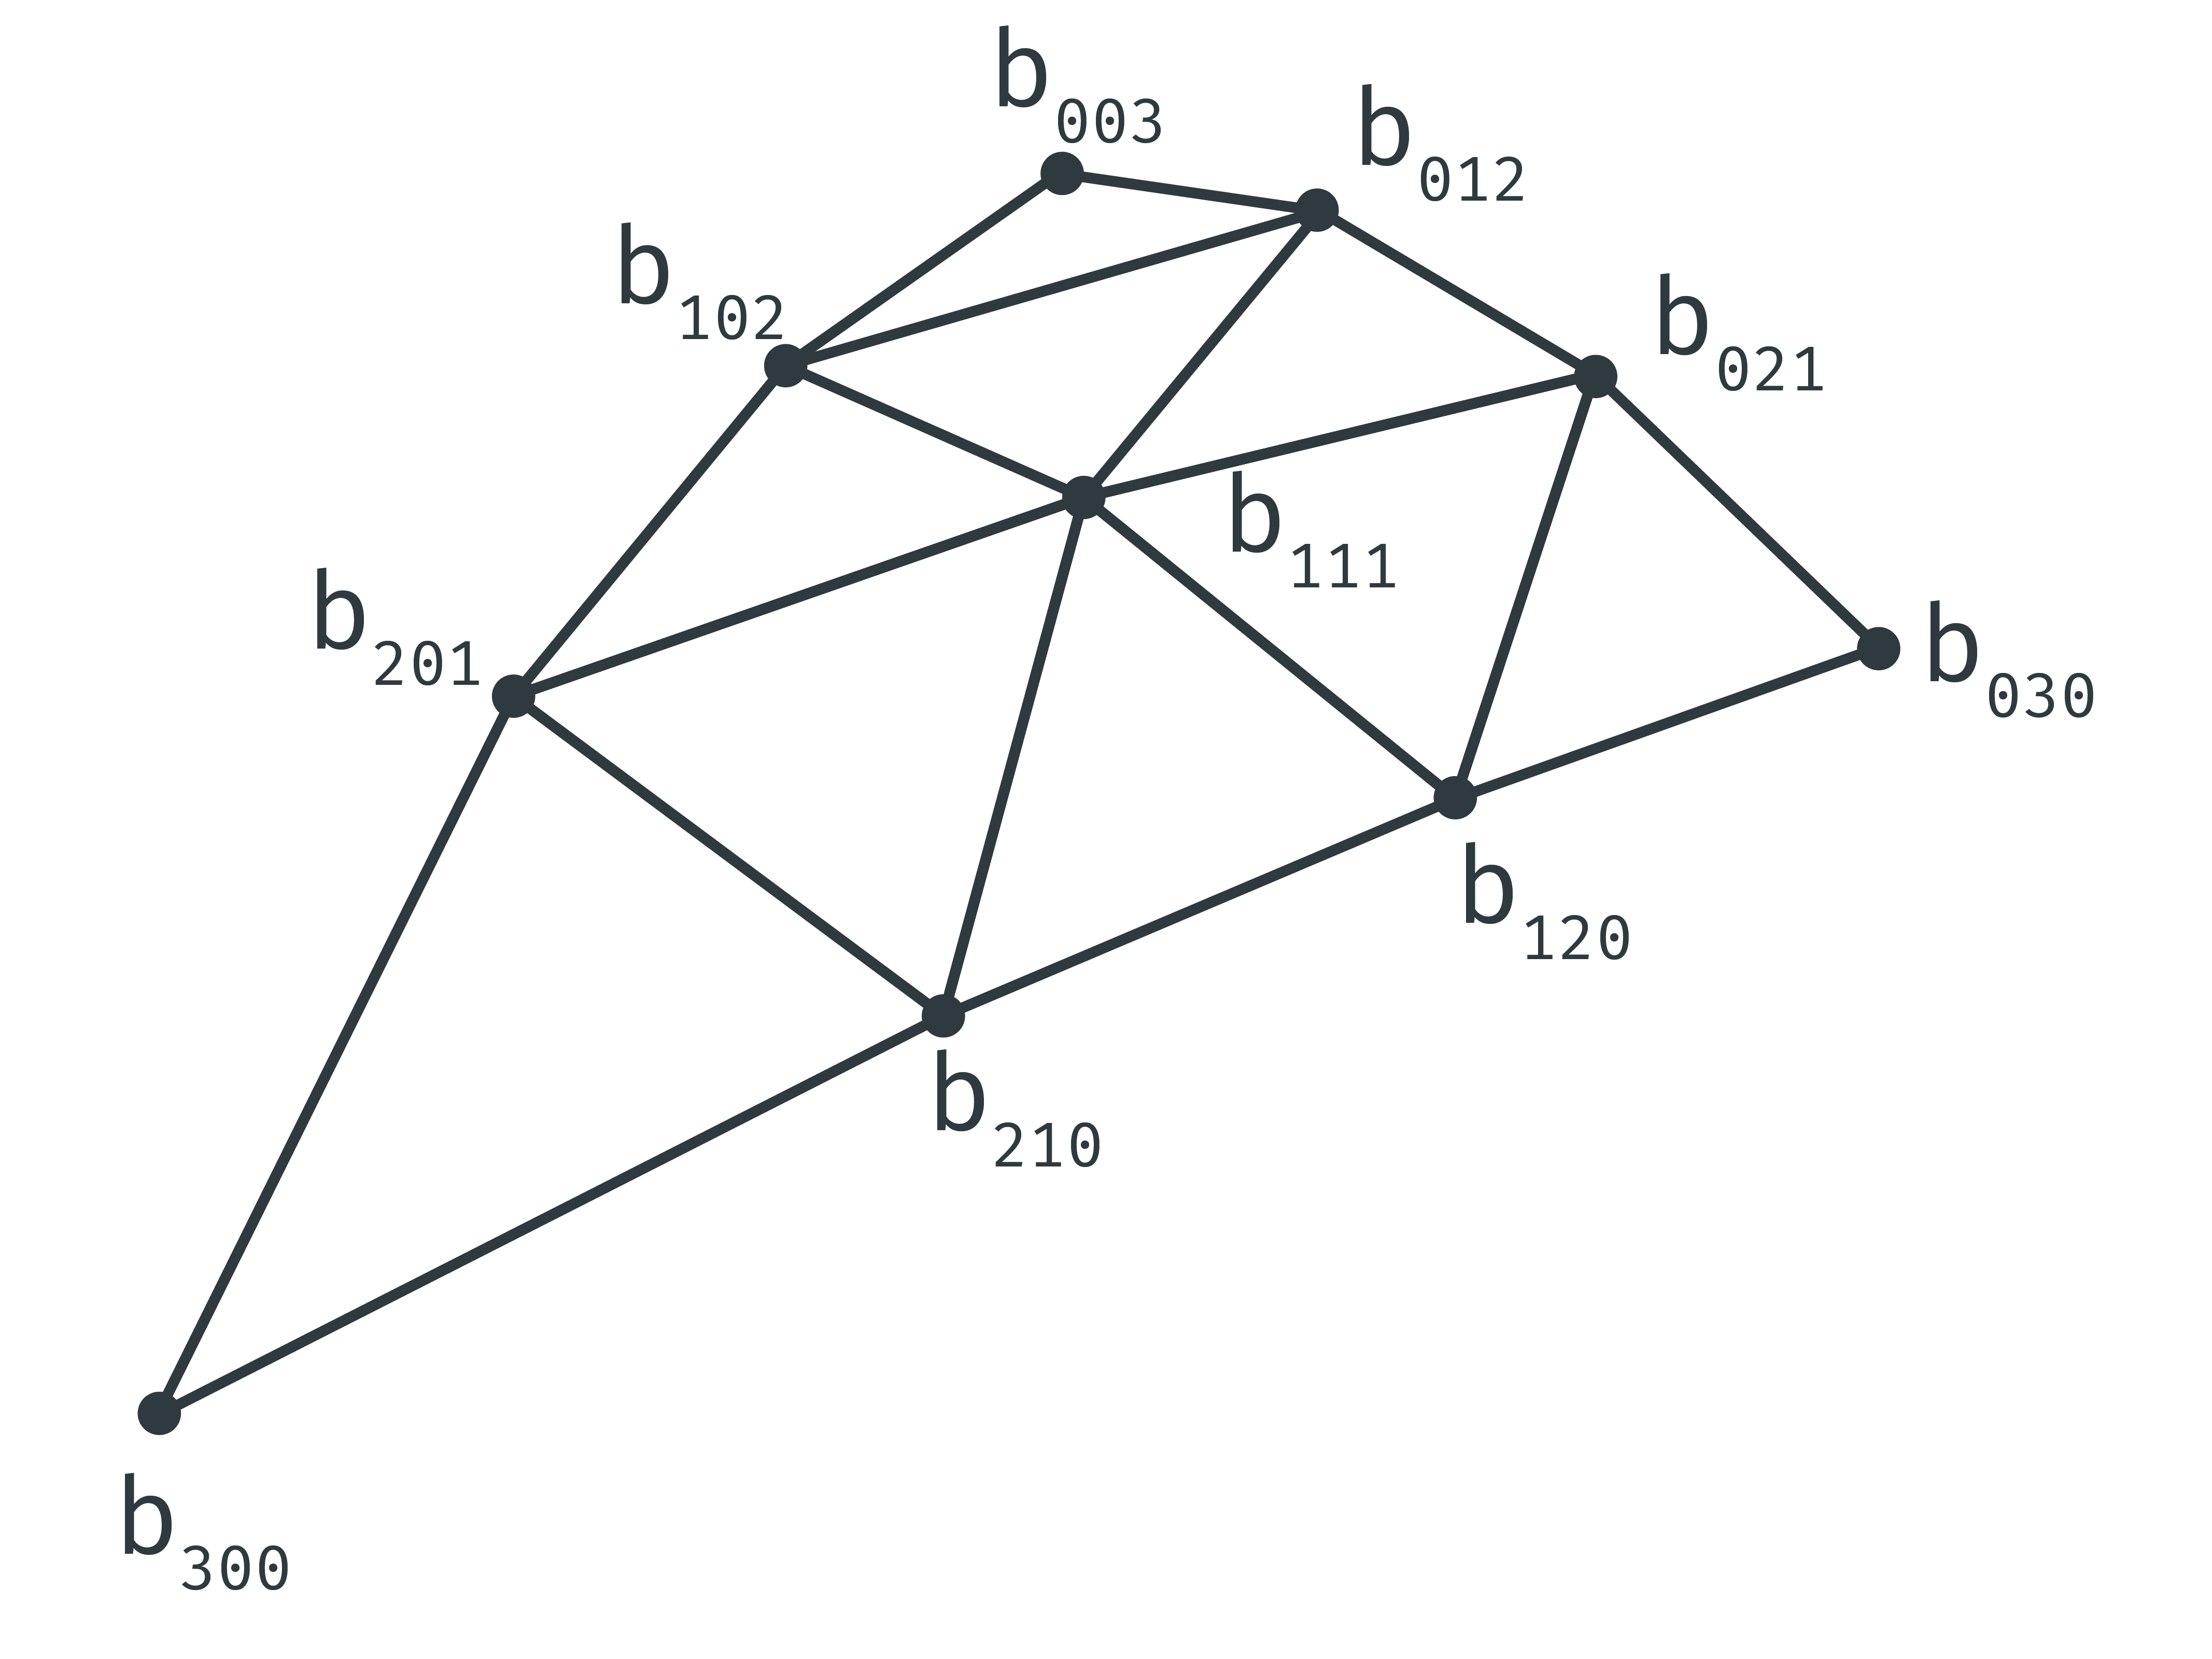
\includegraphics[width=0.45\textwidth]{./content/img/method/geometry.png}
	\caption{The geometric component: the control net of a triangular B\`ezier patch.}
	\label{fig:method:control_net}
\end{figure}
%
% ## Geometric component defined by triangluar cubic Bezier patch.
%
In the next subsection we discuss the definition of the geometry of a PN triangle. Next in subsection \ref{sss:control_point_construction} we discuss the construction of the control points necessary for defining the geometry. 

\subsubsection{Basic form}
The geometric component of a PN triangle is defined by a triangular cubic B\`ezier patch. Such a patch $b$ is defines as follows:
%
\begin{align}
\noalign{$b: \quad R^2 \mapsto R^3,\quad$ for $w = 1 - u - v, \quad u, v, w \geq 0$}
\begin{split}\label{eq:method:cubic_bezier_patch}
    b(u,v) ={}& \sum_{i + j + k = 3} b_{ijk}\frac{3!}{i!j!k!} u^i v^j w^k,\\
      	   ={}& b_{300}w^3 + b_{030}u^3 + b_{003}v^3\\
      	    {}& + b_{210}3w^3 + b_{120}3wu^2 + b_{201}3w^2v\\
      	    {}& + b_{021}3u^2v + b_{102}2wv^2 + b_{012}3uv^2\\
      	    {}& + b_{111}6wuv.
\end{split}
\end{align}
%
The $b_{ijk}$ variables in equation \ref{eq:method:cubic_bezier_patch} are the control points of the patch (also called coefficients). In figure \ref{fig:method:control_net} the visualization of the network of control points is shown. Thereby we group the coefficients in three different groups, as there construction differs:
%
\begin{align*}
	\text{vertex coefficients: } {}&  b_{300},\ b_{030},\ b_{003} \\
	\text{tangent coefficients: } {}&  b_{210},\ b_{120},\ b_{021},\ b_{012},\ b_{102},\ b_{201}\\
	\text{center coefficient: }   {}&  b_{111}\\
\end{align*}
%
% ## This can be used to triangulated the input primitive and to approximate the cubic bezier patch. Controlled by input tesselation lvl reference to implementation. Barrycentric coordinated and convex combinations.
%
The formula in equation \ref{eq:method:cubic_bezier_patch} can be used to interpolate any point, parameterized by the barycentric coordinates $u$ and $v$ on the patch. This fact is used in the sub-triangulation stage of the rendering process. This is the stage where the cubic B\`ezier surface is approximated by using a number of smaller flat triangles. The number of triangles used for this is determined by the level of detail (or lod). For the original sub-triangulation we refer the reader to the paper of \citeauthor{vlachos2001curved}, because this is where the implementation of this report deviates from the original. Details about this are provided in the implementation section \ref{s:implementation}.
%
% ## Geometry coefficients construction (tangent, vertex, and center) so three cases
%
\subsubsection{Coefficients construction} \label{sss:control_point_construction}
In this section we discuss how the `curved' control net geometry (see figure \ref{fig:method:input_primitive}) is calculated, from the flat input primitive shown in figure \ref{fig:method:input_primitive}. The input primitive provides the the positions $P_1, P_2, P_3 \in \Real^3$ and normals $N_1, N_2, N_3 \in \Real^3$, which are the three corner vertices of the triangle. The coefficients $b_{ijk}$ are computed as follows:
%
\begin{enumerate}
	\item Initially the coefficient $b_{ijk}$ are spread uniformly i.e. the intermediate position of $b_{ijk}$ is given by $(i P_i + j P_2 + kP_3) / 3$.
	\item The vertex coefficients are now in the three corners, so these are left as is.
	\item The tangent coefficients are placed by projecting the intermediate position of the coefficient into the tangent plane of the closest corner. This is illustrated by the image in figure \ref{fig:method:geometry_tangent_projection.png}.
	\item The center coefficient is moved to the average of the tangent coefficients plus $1/2$ the distance it had to travel from its intermediate position.
\end{enumerate}
%
\begin{figure}
	\centering
	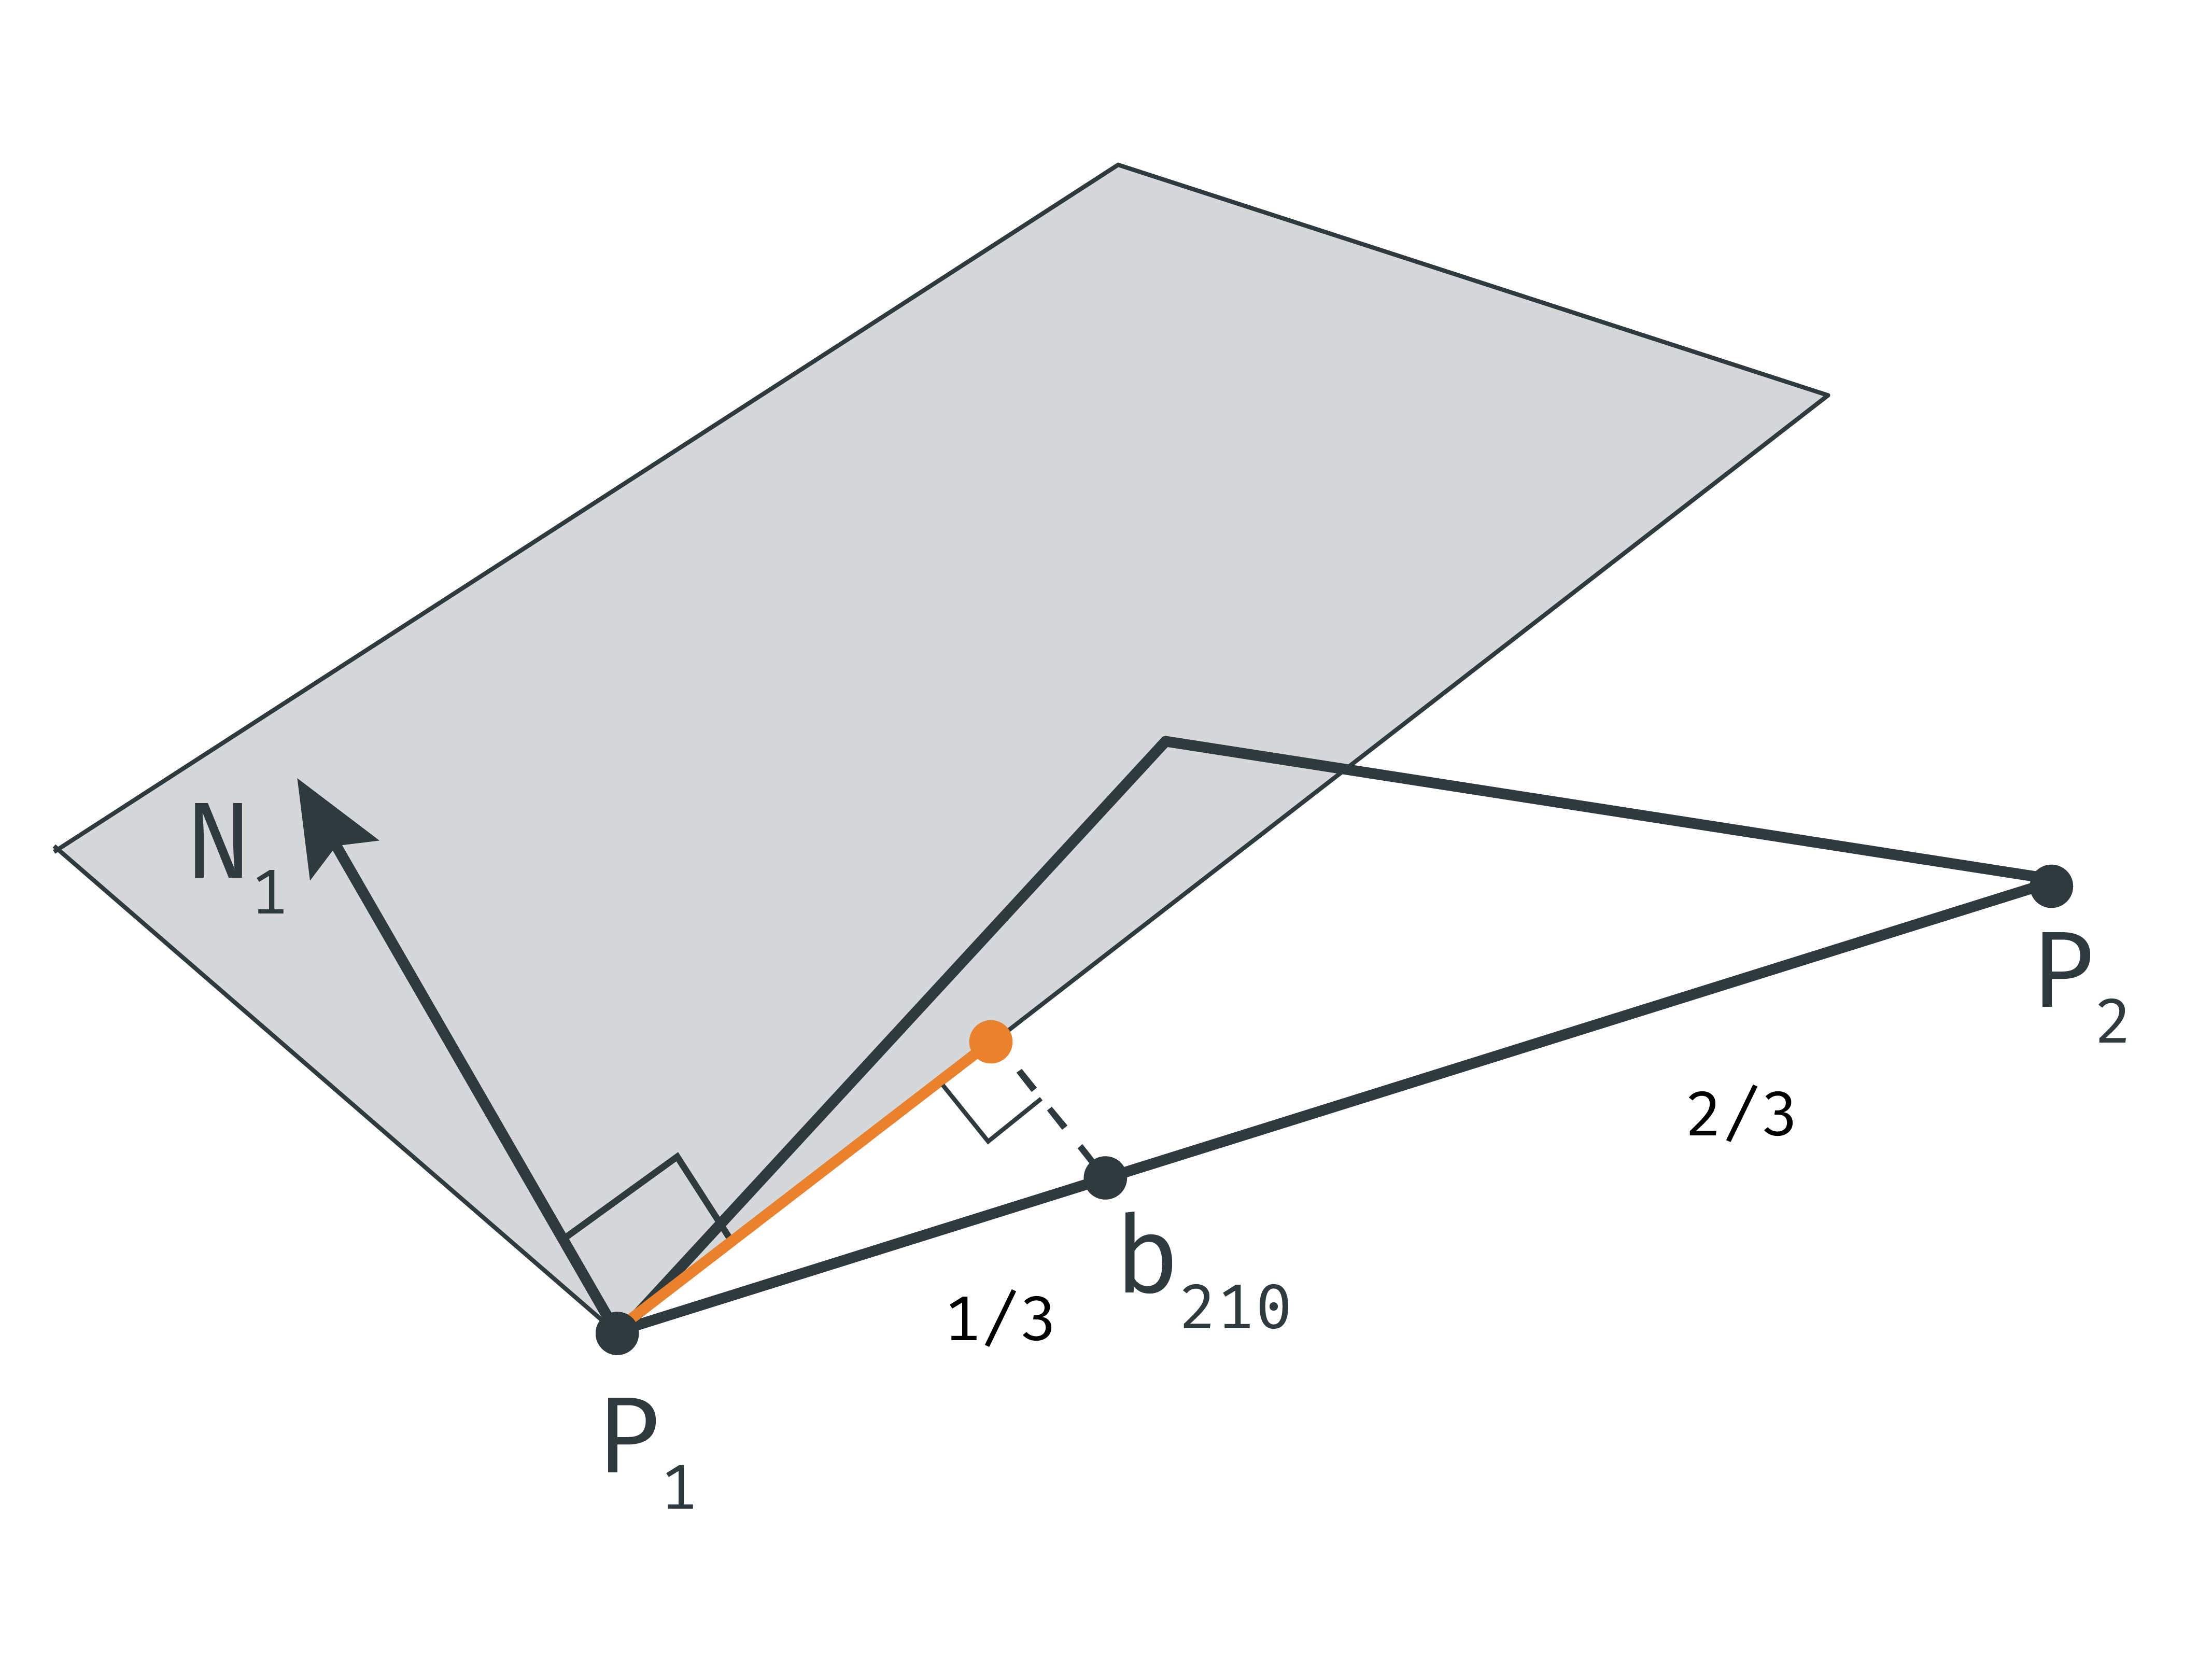
\includegraphics[width=0.45\textwidth]{./content/img/method/geometry_tangent_projection.png}
	\caption{Projection of a tangent coefficient $b_{210}$ to the tangent plane of the closes corner $P_1$.}
	\label{fig:method:geometry_tangent_projection.png}
\end{figure}
%
The following set of formulas describe mathematically how the position of the coefficient can be calculated. For clarity we group together the formulas together in the same way as the coefficients. The vertex coefficients are now given by:
\begin{align}
	b_{300} = P_1,\ b_{030} = P_2,\ b_{003} = P_3
\end{align}
%
% ## Properties of PN triangle geometry bla bla 500 BC verhaal.
%


\todo[inline]{We express geometric compinent as a cubic patch}
\todo[inline]{Discuss parametrization of cubic patch}
\todo[inline]{Discuss the construction of the control points for the cubic patch}